\documentclass[twoside]{book}

% Packages required by doxygen
\usepackage{fixltx2e}
\usepackage{calc}
\usepackage{doxygen}
\usepackage[export]{adjustbox} % also loads graphicx
\usepackage{graphicx}
\usepackage[utf8]{inputenc}
\usepackage{makeidx}
\usepackage{multicol}
\usepackage{multirow}
\PassOptionsToPackage{warn}{textcomp}
\usepackage{textcomp}
\usepackage[nointegrals]{wasysym}
\usepackage[table]{xcolor}

% Font selection
\usepackage[T1]{fontenc}
\usepackage[scaled=.90]{helvet}
\usepackage{courier}
\usepackage{amssymb}
\usepackage{sectsty}
\renewcommand{\familydefault}{\sfdefault}
\allsectionsfont{%
  \fontseries{bc}\selectfont%
  \color{darkgray}%
}
\renewcommand{\DoxyLabelFont}{%
  \fontseries{bc}\selectfont%
  \color{darkgray}%
}
\newcommand{\+}{\discretionary{\mbox{\scriptsize$\hookleftarrow$}}{}{}}

% Page & text layout
\usepackage{geometry}
\geometry{%
  a4paper,%
  top=2.5cm,%
  bottom=2.5cm,%
  left=2.5cm,%
  right=2.5cm%
}
\tolerance=750
\hfuzz=15pt
\hbadness=750
\setlength{\emergencystretch}{15pt}
\setlength{\parindent}{0cm}
\setlength{\parskip}{3ex plus 2ex minus 2ex}
\makeatletter
\renewcommand{\paragraph}{%
  \@startsection{paragraph}{4}{0ex}{-1.0ex}{1.0ex}{%
    \normalfont\normalsize\bfseries\SS@parafont%
  }%
}
\renewcommand{\subparagraph}{%
  \@startsection{subparagraph}{5}{0ex}{-1.0ex}{1.0ex}{%
    \normalfont\normalsize\bfseries\SS@subparafont%
  }%
}
\makeatother

% Headers & footers
\usepackage{fancyhdr}
\pagestyle{fancyplain}
\fancyhead[LE]{\fancyplain{}{\bfseries\thepage}}
\fancyhead[CE]{\fancyplain{}{}}
\fancyhead[RE]{\fancyplain{}{\bfseries\leftmark}}
\fancyhead[LO]{\fancyplain{}{\bfseries\rightmark}}
\fancyhead[CO]{\fancyplain{}{}}
\fancyhead[RO]{\fancyplain{}{\bfseries\thepage}}
\fancyfoot[LE]{\fancyplain{}{}}
\fancyfoot[CE]{\fancyplain{}{}}
\fancyfoot[RE]{\fancyplain{}{\bfseries\scriptsize Generated by Doxygen }}
\fancyfoot[LO]{\fancyplain{}{\bfseries\scriptsize Generated by Doxygen }}
\fancyfoot[CO]{\fancyplain{}{}}
\fancyfoot[RO]{\fancyplain{}{}}
\renewcommand{\footrulewidth}{0.4pt}
\renewcommand{\chaptermark}[1]{%
  \markboth{#1}{}%
}
\renewcommand{\sectionmark}[1]{%
  \markright{\thesection\ #1}%
}

% Indices & bibliography
\usepackage{natbib}
\usepackage[titles]{tocloft}
\setcounter{tocdepth}{3}
\setcounter{secnumdepth}{5}
\makeindex

% Hyperlinks (required, but should be loaded last)
\usepackage{ifpdf}
\ifpdf
  \usepackage[pdftex,pagebackref=true]{hyperref}
\else
  \usepackage[ps2pdf,pagebackref=true]{hyperref}
\fi
\hypersetup{%
  colorlinks=true,%
  linkcolor=blue,%
  citecolor=blue,%
  unicode%
}

% Custom commands
\newcommand{\clearemptydoublepage}{%
  \newpage{\pagestyle{empty}\cleardoublepage}%
}

\usepackage{caption}
\captionsetup{labelsep=space,justification=centering,font={bf},singlelinecheck=off,skip=4pt,position=top}

%===== C O N T E N T S =====

\begin{document}

% Titlepage & ToC
\hypersetup{pageanchor=false,
             bookmarksnumbered=true,
             pdfencoding=unicode
            }
\pagenumbering{alph}
\begin{titlepage}
\vspace*{7cm}
\begin{center}%
{\Large M\+\_\+path }\\
\vspace*{1cm}
{\large Generated by Doxygen 1.8.14}\\
\end{center}
\end{titlepage}
\clearemptydoublepage
\pagenumbering{roman}
\tableofcontents
\clearemptydoublepage
\pagenumbering{arabic}
\hypersetup{pageanchor=true}

%--- Begin generated contents ---
\chapter{M\+\_\+path Fortran Library}
\label{index}\hypertarget{index}{}    

    \hypertarget{index_Introduction}{}\section{Introduction}\label{index_Introduction}
A O\+OP interface to pathname-\/related and file-\/related procedures in the G\+PF (General Purpose Fortran) package

      
\chapter{Modules Index}
\section{Modules List}
Here is a list of all modules with brief descriptions\+:\begin{DoxyCompactList}
\item\contentsline{section}{\mbox{\hyperlink{namespacem__path}{m\+\_\+path}} \\*\subsubsection*{N\+A\+ME}

path(3f) -\/ \mbox{[}M\+\_\+path\mbox{]} O\+OP interface for a G\+NU Linux or Unix pathname (L\+I\+C\+E\+N\+SE\+:PD) \subsubsection*{S\+Y\+N\+O\+P\+S\+IS}}{\pageref{namespacem__path}}{}
\end{DoxyCompactList}

\chapter{Data Type Index}
\section{Data Types List}
Here are the data types with brief descriptions\+:\begin{DoxyCompactList}
\item\contentsline{section}{\mbox{\hyperlink{structm__path_1_1path}{m\+\_\+path\+::path}} }{\pageref{structm__path_1_1path}}{}
\end{DoxyCompactList}

\chapter{File Index}
\section{File List}
Here is a list of all files with brief descriptions\+:\begin{DoxyCompactList}
\item\contentsline{section}{/home/urbanjs/venus/\+V600/github/\+M\+\_\+path/src/\mbox{\hyperlink{M__path_8f90}{M\+\_\+path.\+f90}} }{\pageref{M__path_8f90}}{}
\end{DoxyCompactList}

\chapter{Module Documentation}
\hypertarget{namespacem__path}{}\section{m\+\_\+path Module Reference}
\label{namespacem__path}\index{m\+\_\+path@{m\+\_\+path}}


\subsubsection*{N\+A\+ME}

path(3f) -\/ \mbox{[}M\+\_\+path\mbox{]} O\+OP interface for a G\+NU Linux or Unix pathname (L\+I\+C\+E\+N\+SE\+:PD) \subsubsection*{S\+Y\+N\+O\+P\+S\+IS} 


\subsection*{Data Types}
\begin{DoxyCompactItemize}
\item 
interface \mbox{\hyperlink{structm__path_1_1path}{path}}
\end{DoxyCompactItemize}
\subsection*{Functions/\+Subroutines}
\begin{DoxyCompactItemize}
\item 
type(\mbox{\hyperlink{structm__path_1_1path}{path}}) function \mbox{\hyperlink{namespacem__path_ae223f8623f7a985d4349e08bc7540d53}{construct\+\_\+from\+\_\+dat}} (dat)
\item 
subroutine \mbox{\hyperlink{namespacem__path_ad3027220a3a7decb9dd35ddb41a91250}{init\+\_\+path}} (self, name)
\item 
character(len=\+:) function, allocatable \mbox{\hyperlink{namespacem__path_a33fc3c25b98c7441f230b91ddc9c40ad}{branch}} (self)
\item 
character(len=\+:) function, allocatable \mbox{\hyperlink{namespacem__path_a162b776783f42fc4fe2d3a1b951a1172}{leaf}} (self)
\item 
character(len=\+:) function, allocatable \mbox{\hyperlink{namespacem__path_ac0be359b3514ee777302195a99e583c7}{stem}} (self)
\item 
character(len=\+:) function, allocatable \mbox{\hyperlink{namespacem__path_abd678716fe9c893161b30bc80a466097}{bud}} (self)
\item 
character(len=\+:) function, allocatable \mbox{\hyperlink{namespacem__path_a54bcb3564054f6540a65dc32354f2a2d}{path\+\_\+realpath}} (self)
\item 
integer(kind=int64) function, dimension(14) \mbox{\hyperlink{namespacem__path_a44b09269412e4291dce9ce87de5f6d8f}{path\+\_\+stat}} (self)
\item 
logical function \mbox{\hyperlink{namespacem__path_a9e5b51fcb0d98f8a711b9bfbcaa39c66}{path\+\_\+readable}} (self)
\item 
logical function \mbox{\hyperlink{namespacem__path_a27ad0b81b3aedd309035fe3dc4d69128}{path\+\_\+writable}} (self)
\item 
logical function \mbox{\hyperlink{namespacem__path_abcf12fcdc2f3d90663783ff774b25261}{path\+\_\+executable}} (self)
\item 
logical function \mbox{\hyperlink{namespacem__path_a1d3741add7dd7d180b71295c4a1761c6}{path\+\_\+exists}} (self)
\item 
logical function \mbox{\hyperlink{namespacem__path_a4e56f4f3db67378cb4f20340a14f4a0f}{path\+\_\+isdir}} (self)
\item 
logical function \mbox{\hyperlink{namespacem__path_ac073eb26c4277f48777df68b8e2dfcfd}{eq}} (self, other)
\end{DoxyCompactItemize}


\subsection{Detailed Description}
\subsubsection*{N\+A\+ME}

path(3f) -\/ \mbox{[}M\+\_\+path\mbox{]} O\+OP interface for a G\+NU Linux or Unix pathname (L\+I\+C\+E\+N\+SE\+:PD) \subsubsection*{S\+Y\+N\+O\+P\+S\+IS}

type path

! C\+O\+M\+P\+O\+N\+E\+N\+TS\+: character(len=\+:),allocatable \+:\+: name contains

! M\+E\+T\+H\+O\+DS\+: procedure \+:\+: branch procedure \+:\+: leaf procedure \+:\+: stem procedure \+:\+: bud procedure \+:\+: init procedure \+:\+: is\+\_\+dir procedure \+:\+: stat procedure \+:\+: readable procedure \+:\+: writable procedure \+:\+: executable procedure \+:\+: exists procedure \+:\+: realpath

! O\+V\+E\+R\+L\+O\+A\+D\+ED O\+P\+E\+R\+A\+T\+O\+RS F\+OR T\+Y\+P\+E(path) procedure,private \+:\+: eq generic \+:\+: operator(==) =$>$ eq end type path

\subsubsection*{D\+E\+S\+C\+R\+I\+P\+T\+I\+ON}

Given a pathname, resolve or expand it into branch/stem.\+bud and/or branch/leaf, test for file type and access privileges if file exists, and return system statistics.

Assumes directory separator is a slash (\textquotesingle{}/\textquotesingle{}) and that filename does not contain trailing spaces.

/branch/leaf /branch/stem.bud

\subsubsection*{O\+P\+T\+I\+O\+NS}

F\+I\+L\+E\+N\+A\+ME pathname

\subsubsection*{R\+E\+T\+U\+R\+NS}

name name of file

branch() Output F\+I\+L\+E\+N\+A\+ME with its last non-\/slash component and trailing slashes removed. if F\+I\+L\+E\+N\+A\+ME contains no \textquotesingle{}/\textquotesingle{} character, output \char`\"{}.\char`\"{} (meaning the current directory).

leaf() Output F\+I\+L\+E\+N\+A\+ME with anything up to and including the right-\/most slashes removed. stem() Output F\+I\+L\+E\+N\+A\+ME leaf with any right-\/most suffix removed. A suffix is anything from the rightmost period in the filename leaf to the end of the pathname. bud() Output F\+I\+L\+E\+N\+A\+ME right-\/most suffix.

is\+\_\+dir() a logical specifying if path is currently a directory pathname. exists() determine if file exists readable() determine if file is readable writable() determine if file is writable executable() determine if file is executable

stat() an array of integers describing the current status of the file. returns the same data array as the S\+Y\+S\+T\+E\+M\+\_\+\+S\+T\+A\+T(3f) function with the difference that the status of the call is element 14.

realpath() resolve the pathname using the Posix C routine realpath(3c)

\subsubsection*{E\+X\+A\+M\+P\+LE}

Sample program\+:

program demo\+\_\+path use M\+\_\+path, only \+: path use M\+\_\+system, only \+: system\+\_\+getpwuid, system\+\_\+getgrgid use M\+\_\+time, only \+: fmtdate, u2d use,intrinsic \+:\+: iso\+\_\+fortran\+\_\+env, only \+: int8, int16, int32, int64, real32, real64, real128 character(len=$\ast$),parameter \+:\+: fmt\+\_\+date=\textquotesingle{}year-\/month-\/day hour\+:minute\+:second\textquotesingle{} type(path) \+:\+: file character(len=\+:),allocatable \+:\+: filename integer(kind=int64) \+:\+: buff(14) integer \+:\+: i do i = 1 , max(1,command\+\_\+argument\+\_\+count()) if(command\+\_\+argument\+\_\+count().eq.\+0)then filename=\textquotesingle{}.\textquotesingle{} else call getname(i,filename) endif

filename=filename ! or call fileinit(filename)

deallocate(filename) ! write($\ast$,$\ast$)\textquotesingle{}name........ \textquotesingle{},filename write($\ast$,$\ast$)\textquotesingle{}branch...... \textquotesingle{},filebranch() write($\ast$,$\ast$)\textquotesingle{}leaf........ \textquotesingle{},fileleaf() write($\ast$,$\ast$)\textquotesingle{}stem........ \textquotesingle{},filestem() write($\ast$,$\ast$)\textquotesingle{}bud......... \textquotesingle{},filebud() write($\ast$,$\ast$)\textquotesingle{}is\+\_\+dir...... \textquotesingle{},fileis\+\_\+dir() write($\ast$,$\ast$)\textquotesingle{}readable.... \textquotesingle{},filereadable() write($\ast$,$\ast$)\textquotesingle{}writable.... \textquotesingle{},filewritable() write($\ast$,$\ast$)\textquotesingle{}executable.. \textquotesingle{},fileexecutable() write($\ast$,$\ast$)\textquotesingle{}exists...... \textquotesingle{},fileexists() write($\ast$,$\ast$)\textquotesingle{}realpath.... \textquotesingle{},filerealpath() write($\ast$,$\ast$)\textquotesingle{}stat........ \textquotesingle{} buff=filestat() if(buff(14) == 0) then write ($\ast$, F\+MT=\char`\"{}(9x,\textquotesingle{}\+Device I\+D(hex/decimal)\+:\textquotesingle{},      T40, Z0,\textquotesingle{}h/\textquotesingle{},\+I0,\textquotesingle{}d\textquotesingle{})\char`\"{}) buff(1),buff(1) write ($\ast$, F\+MT=\char`\"{}(9x,\textquotesingle{}\+Inode number\+:\textquotesingle{},                T40, I0)\char`\"{}) buff(2) write ($\ast$, F\+MT=\char`\"{}(9x,\textquotesingle{}\+File mode (octal)\+:\textquotesingle{},           T40, O19)\char`\"{}) buff(3) write ($\ast$, F\+MT=\char`\"{}(9x,\textquotesingle{}\+Number of links\+:\textquotesingle{},             T40, I0)\char`\"{}) buff(4) write ($\ast$, F\+MT=\char`\"{}(9x,\textquotesingle{}\+Owner\textquotesingle{}\textquotesingle{}s uid/username\+:\textquotesingle{},       T40, I0,1x, A)\char`\"{}) buff(5), system\+\_\+getpwuid(buff(5)) write ($\ast$, F\+MT=\char`\"{}(9x,\textquotesingle{}\+Owner\textquotesingle{}\textquotesingle{}s gid/group\+:\textquotesingle{},          T40, I0,1x, A)\char`\"{}) buff(6), system\+\_\+getgrgid(buff(6)) write ($\ast$, F\+MT=\char`\"{}(9x,\textquotesingle{}\+Device where located\+:\textquotesingle{},        T40, I0)\char`\"{}) buff(7) write ($\ast$, F\+MT=\char`\"{}(9x,\textquotesingle{}\+File size(bytes)\+:\textquotesingle{},            T40, I0)\char`\"{}) buff(8) write ($\ast$, F\+MT=\char`\"{}(9x,\textquotesingle{}\+Last access time\+:\textquotesingle{},            T40, I0,1x, A)\char`\"{}) buff(9), fmtdate(u2d(int(buff(9))),fmt\+\_\+date) write ($\ast$, F\+MT=\char`\"{}(9x,\textquotesingle{}\+Last modification time\+:\textquotesingle{},      T40, I0,1x, A)\char`\"{}) buff(10),fmtdate(u2d(int(buff(10))),fmt\+\_\+date) write ($\ast$, F\+MT=\char`\"{}(9x,\textquotesingle{}\+Last status change time\+:\textquotesingle{},     T40, I0,1x, A)\char`\"{}) buff(11),fmtdate(u2d(int(buff(11))),fmt\+\_\+date) write ($\ast$, F\+MT=\char`\"{}(9x,\textquotesingle{}\+Preferred block size(bytes)\+:\textquotesingle{}, T40, I0)\char`\"{}) buff(12) write ($\ast$, F\+MT=\char`\"{}(9x,\textquotesingle{}\+No. of blocks allocated\+:\textquotesingle{},     T40, I0)\char`\"{}) buff(13) else write ($\ast$,$\ast$) \textquotesingle{}{\itshape pathstat} error\+: \textquotesingle{},filename,\textquotesingle{} status= \textquotesingle{},status endif write($\ast$,$\ast$) enddo

contains subroutine getname(i,fn) integer,intent(in) \+:\+: i character(len=\+:),allocatable,intent(out) \+:\+: fn integer \+:\+: fn\+\_\+length ! get pathname from command line arguments call get\+\_\+command\+\_\+argument (i , length=fn\+\_\+length) allocate(character(len=fn\+\_\+length) \+:\+: fn) call get\+\_\+command\+\_\+argument (i , value=fn) end subroutine getname end program demo\+\_\+path Results\+:

Sample program executions\+:

demo\+\_\+path \$\+H\+O\+ME \$\+H\+O\+ME/.bashrc

name........ /home/urbanjs/\+V600 branch...... /home/urbanjs leaf........ V600 stem........ V600 bud......... is\+\_\+dir...... T readable.... T writable... T executable.. T exists...... T realpath.... /home/urbanjs/\+V600 stat........ Device ID(hex/decimal)\+: 3\+E6\+B\+E045h/1047257157d Inode number\+: 281474977443215 File mode (octal)\+: 40700 Number of links\+: 1 Owner\textquotesingle{}s uid/username\+: 197609 J\+SU Owner\textquotesingle{}s gid/group\+: 197121 None Device where located\+: 0 File size(bytes)\+: 0 Last access time\+: 1559495702 2019-\/06-\/02 13\+:15\+:02 Last modification time\+: 1559495702 2019-\/06-\/02 13\+:15\+:02 Last status change time\+: 1559495702 2019-\/06-\/02 13\+:15\+:02 Preferred block size(bytes)\+: 65536 No. of blocks allocated\+: 92

name........ /home/urbanjs/\+V600/.bashrc branch...... /home/urbanjs/\+V600 leaf........ .bashrc stem........ .bashrc bud......... is\+\_\+dir...... F readable.... T writable... T executable.. T exists...... T realpath.... /home/urbanjs/\+V600/.bashrc stat........ Device ID(hex/decimal)\+: 3\+E6\+B\+E045h/1047257157d Inode number\+: 59672695062674129 File mode (octal)\+: 100744 Number of links\+: 1 Owner\textquotesingle{}s uid/username\+: 197609 J\+SU Owner\textquotesingle{}s gid/group\+: 4294967295 Unknown+\+Group Device where located\+: 0 File size(bytes)\+: 8744 Last access time\+: 1434310665 2015-\/06-\/14 15\+:37\+:45 Last modification time\+: 1533428694 2018-\/08-\/04 20\+:24\+:54 Last status change time\+: 1533428694 2018-\/08-\/04 20\+:24\+:54 Preferred block size(bytes)\+: 65536 No. of blocks allocated\+: 12

\subsubsection*{A\+U\+T\+H\+OR}

John S. Urban

\subsubsection*{L\+I\+C\+E\+N\+SE}

Public Domain 

\subsection{Function/\+Subroutine Documentation}
\mbox{\Hypertarget{namespacem__path_a33fc3c25b98c7441f230b91ddc9c40ad}\label{namespacem__path_a33fc3c25b98c7441f230b91ddc9c40ad}} 
\index{m\+\_\+path@{m\+\_\+path}!branch@{branch}}
\index{branch@{branch}!m\+\_\+path@{m\+\_\+path}}
\subsubsection{\texorpdfstring{branch()}{branch()}}
{\footnotesize\ttfamily character(len=\+:) function, allocatable m\+\_\+path\+::branch (\begin{DoxyParamCaption}\item[{class(\mbox{\hyperlink{structm__path_1_1path}{path}}), intent(in)}]{self }\end{DoxyParamCaption})\hspace{0.3cm}{\ttfamily [private]}}

\mbox{\Hypertarget{namespacem__path_abd678716fe9c893161b30bc80a466097}\label{namespacem__path_abd678716fe9c893161b30bc80a466097}} 
\index{m\+\_\+path@{m\+\_\+path}!bud@{bud}}
\index{bud@{bud}!m\+\_\+path@{m\+\_\+path}}
\subsubsection{\texorpdfstring{bud()}{bud()}}
{\footnotesize\ttfamily character(len=\+:) function, allocatable m\+\_\+path\+::bud (\begin{DoxyParamCaption}\item[{class(\mbox{\hyperlink{structm__path_1_1path}{path}}), intent(in)}]{self }\end{DoxyParamCaption})\hspace{0.3cm}{\ttfamily [private]}}

\mbox{\Hypertarget{namespacem__path_ae223f8623f7a985d4349e08bc7540d53}\label{namespacem__path_ae223f8623f7a985d4349e08bc7540d53}} 
\index{m\+\_\+path@{m\+\_\+path}!construct\+\_\+from\+\_\+dat@{construct\+\_\+from\+\_\+dat}}
\index{construct\+\_\+from\+\_\+dat@{construct\+\_\+from\+\_\+dat}!m\+\_\+path@{m\+\_\+path}}
\subsubsection{\texorpdfstring{construct\+\_\+from\+\_\+dat()}{construct\_from\_dat()}}
{\footnotesize\ttfamily type(\mbox{\hyperlink{structm__path_1_1path}{path}}) function m\+\_\+path\+::construct\+\_\+from\+\_\+dat (\begin{DoxyParamCaption}\item[{character(len=$\ast$), intent(in)}]{dat }\end{DoxyParamCaption})\hspace{0.3cm}{\ttfamily [private]}}

Here is the caller graph for this function\+:\nopagebreak
\begin{figure}[H]
\begin{center}
\leavevmode
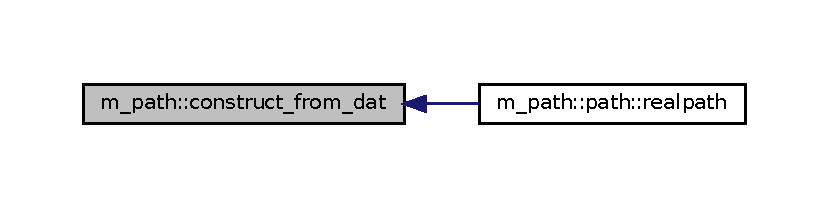
\includegraphics[width=350pt]{namespacem__path_ae223f8623f7a985d4349e08bc7540d53_icgraph}
\end{center}
\end{figure}
\mbox{\Hypertarget{namespacem__path_ac073eb26c4277f48777df68b8e2dfcfd}\label{namespacem__path_ac073eb26c4277f48777df68b8e2dfcfd}} 
\index{m\+\_\+path@{m\+\_\+path}!eq@{eq}}
\index{eq@{eq}!m\+\_\+path@{m\+\_\+path}}
\subsubsection{\texorpdfstring{eq()}{eq()}}
{\footnotesize\ttfamily logical function m\+\_\+path\+::eq (\begin{DoxyParamCaption}\item[{class(\mbox{\hyperlink{structm__path_1_1path}{path}}), intent(in)}]{self,  }\item[{type(\mbox{\hyperlink{structm__path_1_1path}{path}}), intent(in)}]{other }\end{DoxyParamCaption})\hspace{0.3cm}{\ttfamily [private]}}

\mbox{\Hypertarget{namespacem__path_ad3027220a3a7decb9dd35ddb41a91250}\label{namespacem__path_ad3027220a3a7decb9dd35ddb41a91250}} 
\index{m\+\_\+path@{m\+\_\+path}!init\+\_\+path@{init\+\_\+path}}
\index{init\+\_\+path@{init\+\_\+path}!m\+\_\+path@{m\+\_\+path}}
\subsubsection{\texorpdfstring{init\+\_\+path()}{init\_path()}}
{\footnotesize\ttfamily subroutine m\+\_\+path\+::init\+\_\+path (\begin{DoxyParamCaption}\item[{class(\mbox{\hyperlink{structm__path_1_1path}{path}})}]{self,  }\item[{character(len=$\ast$), intent(in), optional}]{name }\end{DoxyParamCaption})\hspace{0.3cm}{\ttfamily [private]}}

\mbox{\Hypertarget{namespacem__path_a162b776783f42fc4fe2d3a1b951a1172}\label{namespacem__path_a162b776783f42fc4fe2d3a1b951a1172}} 
\index{m\+\_\+path@{m\+\_\+path}!leaf@{leaf}}
\index{leaf@{leaf}!m\+\_\+path@{m\+\_\+path}}
\subsubsection{\texorpdfstring{leaf()}{leaf()}}
{\footnotesize\ttfamily character(len=\+:) function, allocatable m\+\_\+path\+::leaf (\begin{DoxyParamCaption}\item[{class(\mbox{\hyperlink{structm__path_1_1path}{path}}), intent(in)}]{self }\end{DoxyParamCaption})}

\mbox{\Hypertarget{namespacem__path_abcf12fcdc2f3d90663783ff774b25261}\label{namespacem__path_abcf12fcdc2f3d90663783ff774b25261}} 
\index{m\+\_\+path@{m\+\_\+path}!path\+\_\+executable@{path\+\_\+executable}}
\index{path\+\_\+executable@{path\+\_\+executable}!m\+\_\+path@{m\+\_\+path}}
\subsubsection{\texorpdfstring{path\+\_\+executable()}{path\_executable()}}
{\footnotesize\ttfamily logical function m\+\_\+path\+::path\+\_\+executable (\begin{DoxyParamCaption}\item[{class(\mbox{\hyperlink{structm__path_1_1path}{path}}), intent(in)}]{self }\end{DoxyParamCaption})\hspace{0.3cm}{\ttfamily [private]}}

\mbox{\Hypertarget{namespacem__path_a1d3741add7dd7d180b71295c4a1761c6}\label{namespacem__path_a1d3741add7dd7d180b71295c4a1761c6}} 
\index{m\+\_\+path@{m\+\_\+path}!path\+\_\+exists@{path\+\_\+exists}}
\index{path\+\_\+exists@{path\+\_\+exists}!m\+\_\+path@{m\+\_\+path}}
\subsubsection{\texorpdfstring{path\+\_\+exists()}{path\_exists()}}
{\footnotesize\ttfamily logical function m\+\_\+path\+::path\+\_\+exists (\begin{DoxyParamCaption}\item[{class(\mbox{\hyperlink{structm__path_1_1path}{path}}), intent(in)}]{self }\end{DoxyParamCaption})\hspace{0.3cm}{\ttfamily [private]}}

\mbox{\Hypertarget{namespacem__path_a4e56f4f3db67378cb4f20340a14f4a0f}\label{namespacem__path_a4e56f4f3db67378cb4f20340a14f4a0f}} 
\index{m\+\_\+path@{m\+\_\+path}!path\+\_\+isdir@{path\+\_\+isdir}}
\index{path\+\_\+isdir@{path\+\_\+isdir}!m\+\_\+path@{m\+\_\+path}}
\subsubsection{\texorpdfstring{path\+\_\+isdir()}{path\_isdir()}}
{\footnotesize\ttfamily logical function m\+\_\+path\+::path\+\_\+isdir (\begin{DoxyParamCaption}\item[{class(\mbox{\hyperlink{structm__path_1_1path}{path}}), intent(in)}]{self }\end{DoxyParamCaption})\hspace{0.3cm}{\ttfamily [private]}}

\mbox{\Hypertarget{namespacem__path_a9e5b51fcb0d98f8a711b9bfbcaa39c66}\label{namespacem__path_a9e5b51fcb0d98f8a711b9bfbcaa39c66}} 
\index{m\+\_\+path@{m\+\_\+path}!path\+\_\+readable@{path\+\_\+readable}}
\index{path\+\_\+readable@{path\+\_\+readable}!m\+\_\+path@{m\+\_\+path}}
\subsubsection{\texorpdfstring{path\+\_\+readable()}{path\_readable()}}
{\footnotesize\ttfamily logical function m\+\_\+path\+::path\+\_\+readable (\begin{DoxyParamCaption}\item[{class(\mbox{\hyperlink{structm__path_1_1path}{path}}), intent(in)}]{self }\end{DoxyParamCaption})\hspace{0.3cm}{\ttfamily [private]}}

\mbox{\Hypertarget{namespacem__path_a54bcb3564054f6540a65dc32354f2a2d}\label{namespacem__path_a54bcb3564054f6540a65dc32354f2a2d}} 
\index{m\+\_\+path@{m\+\_\+path}!path\+\_\+realpath@{path\+\_\+realpath}}
\index{path\+\_\+realpath@{path\+\_\+realpath}!m\+\_\+path@{m\+\_\+path}}
\subsubsection{\texorpdfstring{path\+\_\+realpath()}{path\_realpath()}}
{\footnotesize\ttfamily character(len=\+:) function, allocatable m\+\_\+path\+::path\+\_\+realpath (\begin{DoxyParamCaption}\item[{class(\mbox{\hyperlink{structm__path_1_1path}{path}}), intent(in)}]{self }\end{DoxyParamCaption})\hspace{0.3cm}{\ttfamily [private]}}

\mbox{\Hypertarget{namespacem__path_a44b09269412e4291dce9ce87de5f6d8f}\label{namespacem__path_a44b09269412e4291dce9ce87de5f6d8f}} 
\index{m\+\_\+path@{m\+\_\+path}!path\+\_\+stat@{path\+\_\+stat}}
\index{path\+\_\+stat@{path\+\_\+stat}!m\+\_\+path@{m\+\_\+path}}
\subsubsection{\texorpdfstring{path\+\_\+stat()}{path\_stat()}}
{\footnotesize\ttfamily integer(kind=int64) function, dimension(14) m\+\_\+path\+::path\+\_\+stat (\begin{DoxyParamCaption}\item[{class(\mbox{\hyperlink{structm__path_1_1path}{path}}), intent(in)}]{self }\end{DoxyParamCaption})\hspace{0.3cm}{\ttfamily [private]}}

\mbox{\Hypertarget{namespacem__path_a27ad0b81b3aedd309035fe3dc4d69128}\label{namespacem__path_a27ad0b81b3aedd309035fe3dc4d69128}} 
\index{m\+\_\+path@{m\+\_\+path}!path\+\_\+writable@{path\+\_\+writable}}
\index{path\+\_\+writable@{path\+\_\+writable}!m\+\_\+path@{m\+\_\+path}}
\subsubsection{\texorpdfstring{path\+\_\+writable()}{path\_writable()}}
{\footnotesize\ttfamily logical function m\+\_\+path\+::path\+\_\+writable (\begin{DoxyParamCaption}\item[{class(\mbox{\hyperlink{structm__path_1_1path}{path}}), intent(in)}]{self }\end{DoxyParamCaption})\hspace{0.3cm}{\ttfamily [private]}}

\mbox{\Hypertarget{namespacem__path_ac0be359b3514ee777302195a99e583c7}\label{namespacem__path_ac0be359b3514ee777302195a99e583c7}} 
\index{m\+\_\+path@{m\+\_\+path}!stem@{stem}}
\index{stem@{stem}!m\+\_\+path@{m\+\_\+path}}
\subsubsection{\texorpdfstring{stem()}{stem()}}
{\footnotesize\ttfamily character(len=\+:) function, allocatable m\+\_\+path\+::stem (\begin{DoxyParamCaption}\item[{class(\mbox{\hyperlink{structm__path_1_1path}{path}}), intent(in)}]{self }\end{DoxyParamCaption})}


\chapter{Data Type Documentation}
\hypertarget{structm__path_1_1path}{}\section{m\+\_\+path\+:\+:path Interface Reference}
\label{structm__path_1_1path}\index{m\+\_\+path\+::path@{m\+\_\+path\+::path}}
\subsection*{Private Member Functions}
\begin{DoxyCompactItemize}
\item 
procedure \mbox{\hyperlink{structm__path_1_1path_a51ab53ea8780aa950701aa63de109bb5}{branch}}
\item 
procedure \mbox{\hyperlink{structm__path_1_1path_ac48a286ac54ce081ff8f757bc7724c8d}{leaf}}
\item 
procedure \mbox{\hyperlink{structm__path_1_1path_a9f4b8368bb43f15d23ba5b17b3b3b901}{stem}}
\item 
procedure \mbox{\hyperlink{structm__path_1_1path_a461f618573516bd745e802f829db588a}{bud}}
\item 
procedure \mbox{\hyperlink{structm__path_1_1path_a4072d4f0862ea6a73c0bcea59e356b40}{init}} =$>$ \mbox{\hyperlink{namespacem__path_ad3027220a3a7decb9dd35ddb41a91250}{init\+\_\+path}}
\item 
procedure \mbox{\hyperlink{structm__path_1_1path_ab9edbe441902b825c575010bd1b8a976}{is\+\_\+dir}} =$>$ \mbox{\hyperlink{namespacem__path_a4e56f4f3db67378cb4f20340a14f4a0f}{path\+\_\+isdir}}
\item 
procedure \mbox{\hyperlink{structm__path_1_1path_a69cc8aabf4b8530c82bd133fd641227b}{stat}} =$>$ \mbox{\hyperlink{namespacem__path_a44b09269412e4291dce9ce87de5f6d8f}{path\+\_\+stat}}
\item 
procedure \mbox{\hyperlink{structm__path_1_1path_a008fa6fc2b63421b3c44c41ed3bf0434}{exists}} =$>$ \mbox{\hyperlink{namespacem__path_a1d3741add7dd7d180b71295c4a1761c6}{path\+\_\+exists}}
\item 
procedure \mbox{\hyperlink{structm__path_1_1path_a77ab9b34be0db684654d1f1b375d2f9e}{readable}} =$>$ \mbox{\hyperlink{namespacem__path_a9e5b51fcb0d98f8a711b9bfbcaa39c66}{path\+\_\+readable}}
\item 
procedure \mbox{\hyperlink{structm__path_1_1path_a2769cf5ecff4b5dc0a6b82bd79a18c37}{writable}} =$>$ \mbox{\hyperlink{namespacem__path_a27ad0b81b3aedd309035fe3dc4d69128}{path\+\_\+writable}}
\item 
procedure \mbox{\hyperlink{structm__path_1_1path_aef5ccbd9f037749751a4ece14ab91bc0}{executable}} =$>$ \mbox{\hyperlink{namespacem__path_abcf12fcdc2f3d90663783ff774b25261}{path\+\_\+executable}}
\item 
procedure \mbox{\hyperlink{structm__path_1_1path_a2face141118fc136a54b08f2b46738bb}{realpath}} =$>$ \mbox{\hyperlink{namespacem__path_a54bcb3564054f6540a65dc32354f2a2d}{path\+\_\+realpath}}
\item 
type(\mbox{\hyperlink{structm__path_1_1path}{path}}) function \mbox{\hyperlink{structm__path_1_1path_ae5fad3370033619ca8935281119a38de}{construct\+\_\+from\+\_\+dat}} (dat)
\end{DoxyCompactItemize}
\subsection*{Private Attributes}
\begin{DoxyCompactItemize}
\item 
character(len=\+:), allocatable \mbox{\hyperlink{structm__path_1_1path_a1d9f6aad306106e1032d44c175b80dc4}{name}}
\end{DoxyCompactItemize}


\subsection{Member Function/\+Subroutine Documentation}
\mbox{\Hypertarget{structm__path_1_1path_a51ab53ea8780aa950701aa63de109bb5}\label{structm__path_1_1path_a51ab53ea8780aa950701aa63de109bb5}} 
\index{m\+\_\+path\+::path@{m\+\_\+path\+::path}!branch@{branch}}
\index{branch@{branch}!m\+\_\+path\+::path@{m\+\_\+path\+::path}}
\subsubsection{\texorpdfstring{branch()}{branch()}}
{\footnotesize\ttfamily procedure m\+\_\+path\+::path\+::branch (\begin{DoxyParamCaption}{ }\end{DoxyParamCaption})\hspace{0.3cm}{\ttfamily [private]}}

\mbox{\Hypertarget{structm__path_1_1path_a461f618573516bd745e802f829db588a}\label{structm__path_1_1path_a461f618573516bd745e802f829db588a}} 
\index{m\+\_\+path\+::path@{m\+\_\+path\+::path}!bud@{bud}}
\index{bud@{bud}!m\+\_\+path\+::path@{m\+\_\+path\+::path}}
\subsubsection{\texorpdfstring{bud()}{bud()}}
{\footnotesize\ttfamily procedure m\+\_\+path\+::path\+::bud (\begin{DoxyParamCaption}{ }\end{DoxyParamCaption})\hspace{0.3cm}{\ttfamily [private]}}

\mbox{\Hypertarget{structm__path_1_1path_ae5fad3370033619ca8935281119a38de}\label{structm__path_1_1path_ae5fad3370033619ca8935281119a38de}} 
\index{m\+\_\+path\+::path@{m\+\_\+path\+::path}!construct\+\_\+from\+\_\+dat@{construct\+\_\+from\+\_\+dat}}
\index{construct\+\_\+from\+\_\+dat@{construct\+\_\+from\+\_\+dat}!m\+\_\+path\+::path@{m\+\_\+path\+::path}}
\subsubsection{\texorpdfstring{construct\+\_\+from\+\_\+dat()}{construct\_from\_dat()}}
{\footnotesize\ttfamily type(\mbox{\hyperlink{structm__path_1_1path}{path}}) function m\+\_\+path\+::path\+::construct\+\_\+from\+\_\+dat (\begin{DoxyParamCaption}\item[{character(len=$\ast$), intent(in)}]{dat }\end{DoxyParamCaption})\hspace{0.3cm}{\ttfamily [private]}}

\mbox{\Hypertarget{structm__path_1_1path_aef5ccbd9f037749751a4ece14ab91bc0}\label{structm__path_1_1path_aef5ccbd9f037749751a4ece14ab91bc0}} 
\index{m\+\_\+path\+::path@{m\+\_\+path\+::path}!executable@{executable}}
\index{executable@{executable}!m\+\_\+path\+::path@{m\+\_\+path\+::path}}
\subsubsection{\texorpdfstring{executable()}{executable()}}
{\footnotesize\ttfamily procedure m\+\_\+path\+::path\+::executable (\begin{DoxyParamCaption}{ }\end{DoxyParamCaption})\hspace{0.3cm}{\ttfamily [private]}}

\mbox{\Hypertarget{structm__path_1_1path_a008fa6fc2b63421b3c44c41ed3bf0434}\label{structm__path_1_1path_a008fa6fc2b63421b3c44c41ed3bf0434}} 
\index{m\+\_\+path\+::path@{m\+\_\+path\+::path}!exists@{exists}}
\index{exists@{exists}!m\+\_\+path\+::path@{m\+\_\+path\+::path}}
\subsubsection{\texorpdfstring{exists()}{exists()}}
{\footnotesize\ttfamily procedure m\+\_\+path\+::path\+::exists (\begin{DoxyParamCaption}{ }\end{DoxyParamCaption})\hspace{0.3cm}{\ttfamily [private]}}

\mbox{\Hypertarget{structm__path_1_1path_a4072d4f0862ea6a73c0bcea59e356b40}\label{structm__path_1_1path_a4072d4f0862ea6a73c0bcea59e356b40}} 
\index{m\+\_\+path\+::path@{m\+\_\+path\+::path}!init@{init}}
\index{init@{init}!m\+\_\+path\+::path@{m\+\_\+path\+::path}}
\subsubsection{\texorpdfstring{init()}{init()}}
{\footnotesize\ttfamily procedure m\+\_\+path\+::path\+::init (\begin{DoxyParamCaption}{ }\end{DoxyParamCaption})\hspace{0.3cm}{\ttfamily [private]}}

\mbox{\Hypertarget{structm__path_1_1path_ab9edbe441902b825c575010bd1b8a976}\label{structm__path_1_1path_ab9edbe441902b825c575010bd1b8a976}} 
\index{m\+\_\+path\+::path@{m\+\_\+path\+::path}!is\+\_\+dir@{is\+\_\+dir}}
\index{is\+\_\+dir@{is\+\_\+dir}!m\+\_\+path\+::path@{m\+\_\+path\+::path}}
\subsubsection{\texorpdfstring{is\+\_\+dir()}{is\_dir()}}
{\footnotesize\ttfamily procedure m\+\_\+path\+::path\+::is\+\_\+dir (\begin{DoxyParamCaption}{ }\end{DoxyParamCaption})\hspace{0.3cm}{\ttfamily [private]}}

\mbox{\Hypertarget{structm__path_1_1path_ac48a286ac54ce081ff8f757bc7724c8d}\label{structm__path_1_1path_ac48a286ac54ce081ff8f757bc7724c8d}} 
\index{m\+\_\+path\+::path@{m\+\_\+path\+::path}!leaf@{leaf}}
\index{leaf@{leaf}!m\+\_\+path\+::path@{m\+\_\+path\+::path}}
\subsubsection{\texorpdfstring{leaf()}{leaf()}}
{\footnotesize\ttfamily procedure m\+\_\+path\+::path\+::leaf (\begin{DoxyParamCaption}{ }\end{DoxyParamCaption})\hspace{0.3cm}{\ttfamily [private]}}

\mbox{\Hypertarget{structm__path_1_1path_a77ab9b34be0db684654d1f1b375d2f9e}\label{structm__path_1_1path_a77ab9b34be0db684654d1f1b375d2f9e}} 
\index{m\+\_\+path\+::path@{m\+\_\+path\+::path}!readable@{readable}}
\index{readable@{readable}!m\+\_\+path\+::path@{m\+\_\+path\+::path}}
\subsubsection{\texorpdfstring{readable()}{readable()}}
{\footnotesize\ttfamily procedure m\+\_\+path\+::path\+::readable (\begin{DoxyParamCaption}{ }\end{DoxyParamCaption})\hspace{0.3cm}{\ttfamily [private]}}

\mbox{\Hypertarget{structm__path_1_1path_a2face141118fc136a54b08f2b46738bb}\label{structm__path_1_1path_a2face141118fc136a54b08f2b46738bb}} 
\index{m\+\_\+path\+::path@{m\+\_\+path\+::path}!realpath@{realpath}}
\index{realpath@{realpath}!m\+\_\+path\+::path@{m\+\_\+path\+::path}}
\subsubsection{\texorpdfstring{realpath()}{realpath()}}
{\footnotesize\ttfamily procedure m\+\_\+path\+::path\+::realpath (\begin{DoxyParamCaption}{ }\end{DoxyParamCaption})\hspace{0.3cm}{\ttfamily [private]}}



References m\+\_\+path\+::construct\+\_\+from\+\_\+dat().

Here is the call graph for this function\+:\nopagebreak
\begin{figure}[H]
\begin{center}
\leavevmode
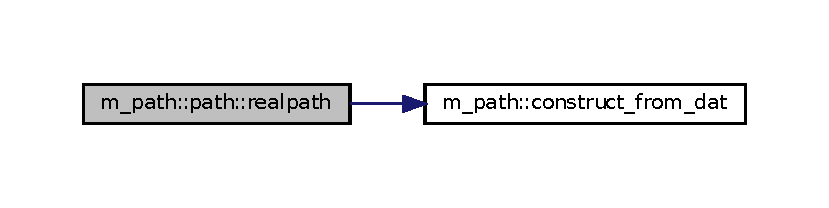
\includegraphics[width=350pt]{structm__path_1_1path_a2face141118fc136a54b08f2b46738bb_cgraph}
\end{center}
\end{figure}
\mbox{\Hypertarget{structm__path_1_1path_a69cc8aabf4b8530c82bd133fd641227b}\label{structm__path_1_1path_a69cc8aabf4b8530c82bd133fd641227b}} 
\index{m\+\_\+path\+::path@{m\+\_\+path\+::path}!stat@{stat}}
\index{stat@{stat}!m\+\_\+path\+::path@{m\+\_\+path\+::path}}
\subsubsection{\texorpdfstring{stat()}{stat()}}
{\footnotesize\ttfamily procedure m\+\_\+path\+::path\+::stat (\begin{DoxyParamCaption}{ }\end{DoxyParamCaption})\hspace{0.3cm}{\ttfamily [private]}}

\mbox{\Hypertarget{structm__path_1_1path_a9f4b8368bb43f15d23ba5b17b3b3b901}\label{structm__path_1_1path_a9f4b8368bb43f15d23ba5b17b3b3b901}} 
\index{m\+\_\+path\+::path@{m\+\_\+path\+::path}!stem@{stem}}
\index{stem@{stem}!m\+\_\+path\+::path@{m\+\_\+path\+::path}}
\subsubsection{\texorpdfstring{stem()}{stem()}}
{\footnotesize\ttfamily procedure m\+\_\+path\+::path\+::stem (\begin{DoxyParamCaption}{ }\end{DoxyParamCaption})\hspace{0.3cm}{\ttfamily [private]}}

\mbox{\Hypertarget{structm__path_1_1path_a2769cf5ecff4b5dc0a6b82bd79a18c37}\label{structm__path_1_1path_a2769cf5ecff4b5dc0a6b82bd79a18c37}} 
\index{m\+\_\+path\+::path@{m\+\_\+path\+::path}!writable@{writable}}
\index{writable@{writable}!m\+\_\+path\+::path@{m\+\_\+path\+::path}}
\subsubsection{\texorpdfstring{writable()}{writable()}}
{\footnotesize\ttfamily procedure m\+\_\+path\+::path\+::writable (\begin{DoxyParamCaption}{ }\end{DoxyParamCaption})\hspace{0.3cm}{\ttfamily [private]}}



\subsection{Member Data Documentation}
\mbox{\Hypertarget{structm__path_1_1path_a1d9f6aad306106e1032d44c175b80dc4}\label{structm__path_1_1path_a1d9f6aad306106e1032d44c175b80dc4}} 
\index{m\+\_\+path\+::path@{m\+\_\+path\+::path}!name@{name}}
\index{name@{name}!m\+\_\+path\+::path@{m\+\_\+path\+::path}}
\subsubsection{\texorpdfstring{name}{name}}
{\footnotesize\ttfamily character(len=\+:), allocatable m\+\_\+path\+::path\+::name\hspace{0.3cm}{\ttfamily [private]}}



The documentation for this interface was generated from the following file\+:\begin{DoxyCompactItemize}
\item 
/home/urbanjs/venus/\+V600/github/\+M\+\_\+path/src/\mbox{\hyperlink{M__path_8f90}{M\+\_\+path.\+f90}}\end{DoxyCompactItemize}

\chapter{File Documentation}
\hypertarget{M__path_8f90}{}\section{/home/urbanjs/venus/\+V600/github/\+M\+\_\+path/src/\+M\+\_\+path.f90 File Reference}
\label{M__path_8f90}\index{/home/urbanjs/venus/\+V600/github/\+M\+\_\+path/src/\+M\+\_\+path.\+f90@{/home/urbanjs/venus/\+V600/github/\+M\+\_\+path/src/\+M\+\_\+path.\+f90}}
\subsection*{Data Types}
\begin{DoxyCompactItemize}
\item 
interface \mbox{\hyperlink{structm__path_1_1path}{m\+\_\+path\+::path}}
\item 
interface \mbox{\hyperlink{structm__path_1_1path}{m\+\_\+path\+::path}}
\end{DoxyCompactItemize}
\subsection*{Modules}
\begin{DoxyCompactItemize}
\item 
module \mbox{\hyperlink{namespacem__path}{m\+\_\+path}}
\begin{DoxyCompactList}\small\item\em \subsubsection*{N\+A\+ME}

path(3f) -\/ \mbox{[}M\+\_\+path\mbox{]} O\+OP interface for a G\+NU Linux or Unix pathname (L\+I\+C\+E\+N\+SE\+:PD) \subsubsection*{S\+Y\+N\+O\+P\+S\+IS}\end{DoxyCompactList}\end{DoxyCompactItemize}
\subsection*{Functions/\+Subroutines}
\begin{DoxyCompactItemize}
\item 
type(path) function \mbox{\hyperlink{namespacem__path_ae223f8623f7a985d4349e08bc7540d53}{m\+\_\+path\+::construct\+\_\+from\+\_\+dat}} (dat)
\item 
subroutine \mbox{\hyperlink{namespacem__path_ad3027220a3a7decb9dd35ddb41a91250}{m\+\_\+path\+::init\+\_\+path}} (self, name)
\item 
character(len=\+:) function, allocatable \mbox{\hyperlink{namespacem__path_a33fc3c25b98c7441f230b91ddc9c40ad}{m\+\_\+path\+::branch}} (self)
\item 
character(len=\+:) function, allocatable \mbox{\hyperlink{namespacem__path_a162b776783f42fc4fe2d3a1b951a1172}{m\+\_\+path\+::leaf}} (self)
\item 
character(len=\+:) function, allocatable \mbox{\hyperlink{namespacem__path_ac0be359b3514ee777302195a99e583c7}{m\+\_\+path\+::stem}} (self)
\item 
character(len=\+:) function, allocatable \mbox{\hyperlink{namespacem__path_abd678716fe9c893161b30bc80a466097}{m\+\_\+path\+::bud}} (self)
\item 
character(len=\+:) function, allocatable \mbox{\hyperlink{namespacem__path_a54bcb3564054f6540a65dc32354f2a2d}{m\+\_\+path\+::path\+\_\+realpath}} (self)
\item 
integer(kind=int64) function, dimension(14) \mbox{\hyperlink{namespacem__path_a44b09269412e4291dce9ce87de5f6d8f}{m\+\_\+path\+::path\+\_\+stat}} (self)
\item 
logical function \mbox{\hyperlink{namespacem__path_a9e5b51fcb0d98f8a711b9bfbcaa39c66}{m\+\_\+path\+::path\+\_\+readable}} (self)
\item 
logical function \mbox{\hyperlink{namespacem__path_a27ad0b81b3aedd309035fe3dc4d69128}{m\+\_\+path\+::path\+\_\+writable}} (self)
\item 
logical function \mbox{\hyperlink{namespacem__path_abcf12fcdc2f3d90663783ff774b25261}{m\+\_\+path\+::path\+\_\+executable}} (self)
\item 
logical function \mbox{\hyperlink{namespacem__path_a1d3741add7dd7d180b71295c4a1761c6}{m\+\_\+path\+::path\+\_\+exists}} (self)
\item 
logical function \mbox{\hyperlink{namespacem__path_a4e56f4f3db67378cb4f20340a14f4a0f}{m\+\_\+path\+::path\+\_\+isdir}} (self)
\item 
logical function \mbox{\hyperlink{namespacem__path_ac073eb26c4277f48777df68b8e2dfcfd}{m\+\_\+path\+::eq}} (self, other)
\end{DoxyCompactItemize}

\hypertarget{mainpage_8txt}{}\section{/home/urbanjs/venus/\+V600/github/\+M\+\_\+path/src/mainpage.txt File Reference}
\label{mainpage_8txt}\index{/home/urbanjs/venus/\+V600/github/\+M\+\_\+path/src/mainpage.\+txt@{/home/urbanjs/venus/\+V600/github/\+M\+\_\+path/src/mainpage.\+txt}}

%--- End generated contents ---

% Index
\backmatter
\newpage
\phantomsection
\clearemptydoublepage
\addcontentsline{toc}{chapter}{Index}
\printindex

\end{document}
